\section{Velocity and Heading Controllers}
\label{s:Velocity_and_Heading_Controllers}
In the previous section, a way point strategy was proposed for path planning of follower vehicles. These way points are used for heading correction which indirectly maintains the lateral offset distance $D_{lat}$ defined by the manned leader. The structure for this heading controller and of a velocity controller for maintaining a longitudinal distance offset will be discussed in this section. 

In section \ref{s:Way_Point_Following} algorithm \ref{alg:WP} produces a way point location for heading correction, $X_{WPC}$, $Y_{WPC}$, at 1 Hz. The heading reference to the heading controller is given by 
\begin{equation}\label{eq:heading_reference}
        \theta_{ref} = \arctan2\Bigg(\frac{Y_{WPC}-Y_{follower}}{X_{WPC}-X_{follower}}\Bigg)
\end{equation}
To regulate this heading a proportional integral controller is used
\begin{equation}\label{eq:heading_controller}
        \alpha(t) = K_{p,\theta}\theta_{error}(t) + \int_{0}^{t}K_{i,\theta}\theta_{error}(t)dt
\end{equation}
where  $\alpha$ is the driver's steering angle, $K_{p,\theta}$ is the proportional heading controller gain, $K_{i,\theta}$ is the integral heading controller gain, and $\theta_{error}(t)$ is the heading error. Since an accurate measurement of tractor heading is assumed from GPS at 10 Hz, the controller is run at the same rate. Figure \ref{fig:Heading_Control_Loop} provides a diagram of the overall controller structure.
\begin{figure}[htb]
    \centering
    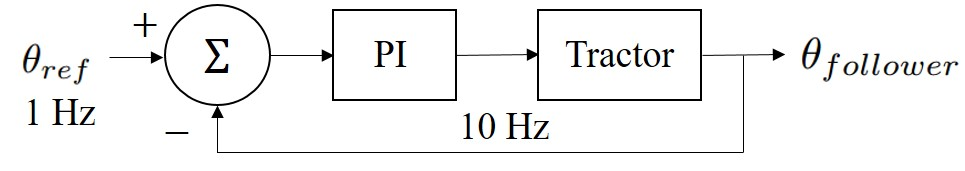
\includegraphics[width=4in]{Heading_Control_Loop}
    \caption{Closed-loop block diagram of the unmanned tractor's heading regulation. The reference input $\theta_{ref}$ is updated at 1 Hz. The PI controller structure is defined in eq. (\ref{eq:heading_controller}) and updates at 10 Hz.}
    \label{fig:Heading_Control_Loop}
\end{figure}
To implement this controller eq. \ref{eq:heading_controller} must be discretized into a difference equation. To do this, the laplace transform is taken where $s$ is the complex laplace variable to give the transfer function
\begin{equation}\label{eq:heading_controller_ctf}
        \frac{\alpha(s)}{\theta_{error}(s)} = K_{p,\theta} + K_{i,\theta}\frac{1}{s}
\end{equation}
To convert this continuous transfer function of the complex variable $s$ into a discrete one of the complex variable $z$, the bilinear transform or tustin approximation is used
\begin{equation}
        z = e^{sT_s} \approx \frac{1+\frac{sT_s}{2}}{1-\frac{sT_s}{2}}
\end{equation}
where $T_s= 0.1$ is the sample time in seconds of the controller. The first order inverse approximation that is substituted for $s$ in eq. \ref{eq:heading_controller_ctf} is
\begin{equation}\label{eq:s2z}
        s \approx \frac{2}{T_s}\frac{1-z^{-1}}{1+z^{-1}}
\end{equation}
The resulting $z$ domain transfer function is then converted back to the time domain using the z transform identify $x[k-k_o] = z^{-k_o}X(z)$ \cite{hansen2014fourier}. The form of the time domain difference equation for a PI controller is given by 
\begin{equation}
    \alpha[k] = -\frac{a_1}{a_0}\alpha[k-1] + \frac{b_0}{a_0}\theta_{error}[k] + \frac{b_1}{b_0}\theta_{error}[k-1]
\end{equation}
This process can be expedited using matlab commands pid, tf, and c2d where pid creates the controller structure, tf converts it to a transfer function, and c2d discretizes the continuous transfer function.

It should be noted that the transfer function between the normalized steering angle, $\alpha$, and the tractor's yaw rate, $\dot\theta$, can be approximated as first order. Using this knowledge, the transfer function between the normalized steering angle and the heading angle can be approximated as
\begin{linenomath*}
    \begin{equation}\label{eq:steer_heading_transfer_function}
        \frac{\theta(s)}{\alpha(s)} = \frac{1}{s}\frac{K_{dc}}{\delta s + 1}
    \end{equation}
\end{linenomath*}
where the DC gain $K_{dc}$ and time constant $\delta$ depend on vehicle velocity and the terrain assuming nominal parameters for differential steering, power-train components are known. This allows for rigorous linear control system design if $K_{dc}$ and $\delta$ are approximated across the vehicle speed range of $[0,4]$ m/s and the terrain parameter space. 

The second low level controller used on follower tractors is for velocity regulation. The previous way point management and selection system and heading controller are responsible for maintaining the manned-leader's specified lateral offset $D_{lat}$ while the velocity controller will be responsible for maintaining a specified longitudinal offset $D_{long}$. The velocity reference for the controller is given by 
\begin{equation}\label{eq:velocity_reference}
        v_{ref} = k_x x_e + v_{leader}
\end{equation}
where $k_x$ is a tunable gain parameter, $x_e$ is the longitudinal error defined in the follower's body fixed frame in the $\mathbf{i}_1$ direction as in \cite{low2015flexible,low2014flexible}, and $v_{leader}$ is the velocity of the manned leader tractor. The parameters $D_{long}$ and $x_{e}$ are illustrated graphically in Fig. \ref{fig:Leader_Follower_Speed_Controller_Error_Diagram} for clarity. Since it is assumed, that tractors recieve GPS signals and can share CAN messages at 10 Hz, the velocity reference input and control loop will also run at this rate.
\begin{figure}[hb]
    \centering
    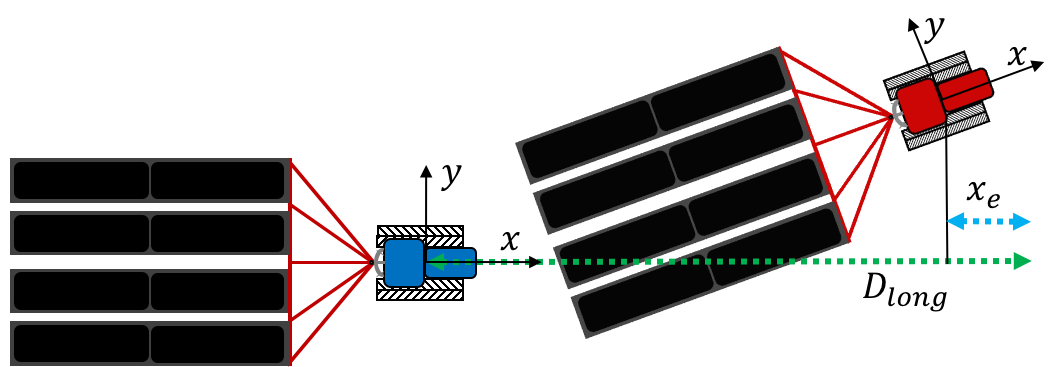
\includegraphics[width=4in]{Leader_Follower_Speed_Controller_Error_Diagram}
    \caption{Diagram of one leader follower pair where the leader and follower are colored red and blue respectively. The longitudinal offset distance to be maintained by the velocity controller $D_{long}$ is denoted with a dotted green line and the error to regulating this distance $x_e$ is shown as a dotted blue line.}
    \label{fig:Leader_Follower_Speed_Controller_Error_Diagram}
\end{figure}
The controller structure and block diagram are given by eq. \ref{eq:speed_controller} and Fig. \ref{fig:Velocity_Control_Loop}
\begin{equation}\label{eq:speed_controller}
    \Pi_{follower} = \Pi_{leader} + K_{p,v}v_e(t) + \int_{0}^{t}K_{i,v}v_e(t)dt
\end{equation}
This controller uses feed-forward inputs from the lead tractor's throttle, $\Pi_{leader}$, and gear selection, $g_{GR,leader}$, in combination with a PI controller for throttle regulation. These feed forward throttle and gear inputs from the leader simplify the controller design and increase robustness since lower gain values can be used for adequate performance. 

The velocity controller is discretized using the same methods as the heading controller where the time domain equation is converted to its laplace transform equivalent, discretized into the $z$ transform, and converted back into the time domain in the form of a difference equation
\begin{equation}
    \Pi_{follower} = \Pi_{leader} + \Pi_{PI}
\end{equation}
\begin{equation}
    \Pi_{PI} = -\frac{a_1}{a_0}\Pi_{PI}[k-1] + \frac{b_0}{a_0}v_e[k] + \frac{b_1}{a_0}v_e[k-1]
\end{equation}
\begin{figure}[htb]
    \centering
    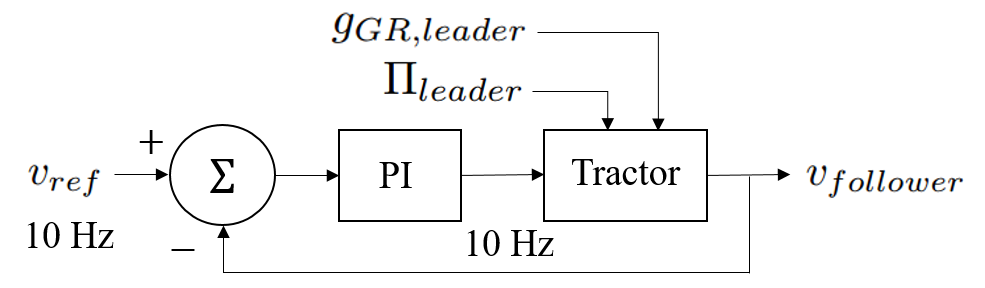
\includegraphics[width=4in]{Velocity_Control_Loop}
    \caption{Closed-loop block diagram of the unmanned tractor's speed. The reference input $v_{ref}$ is updated at 10 Hz. The controller structure is defined in eq. (\ref{eq:speed_controller}) which uses a combination of a PI controller with feed-forward terms $\Pi_{leader}$ and $g_{GR,leader}$ that are the manned leader's throttle and gear selection at 10 Hz.}
    \label{fig:Velocity_Control_Loop}
\end{figure}